\documentclass{beamer}
\mode<presentation>
{
\usepackage{dis-template}
}
\usepackage{listings}
\usepackage{textcomp}
\definecolor{comments}{HTML}{50c878}
\lstset{language=C++,
  basicstyle=\ttfamily,
  keywordstyle=\color{blue}\ttfamily,
  stringstyle=\color{red}\ttfamily,
  commentstyle=\color{comments}\ttfamily,
  breaklines=true
}

\graphicspath{{slides/}} % TODO: eliminate this hack, necessary because scons builds at repository root

%---------------------------------------------------------------------
\titlepageinit{9 (Part 2)}{Embedded Software}{18 \& 19 Feb 2015 (Week 9)}
%---------------------------------------------------------------------
\begin{document}
%---------------------------------------------------------------------
\begin{frame}
\titlepage

\setcounter{tocdepth}{1}
\tableofcontents
\end{frame}

% LAB PREPARATION
% None for this segment

%---------------------------------------------------------------------
\section{Embedded Programming} % [?? mins]
%---------------------------------------------------------------------
\begin{frame}
\centering \huge Embedded Programming
\end{frame}

%---------------------------------------------------------------------
\subsection{Limitations}

\begin{frame}
\frametitle{Hardware Specs}
\begin{columns}[t]
\column{0.646\textwidth}
Recall the hardware specs for your boards:
\vspace{10px}
\begin{itemize}
  \item MKL25Z128VLK4 microcontroller
  \begin{itemize}
    \item 48MHz ARM Cortex-M0+
    \item 128KB flash
    \item 16KB SRAM
  \end{itemize}
\end{itemize}
\vspace{10px}
What might make embedded programming different from desktop programming?

\column{0.323\textwidth}
\begin{figure}
\centering
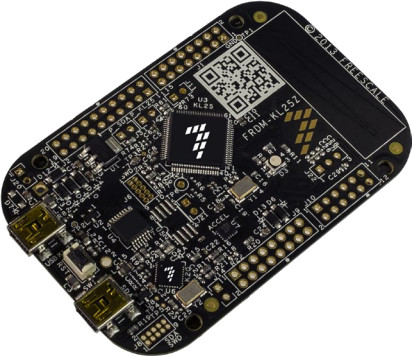
\includegraphics[width=1.0\columnwidth]{images-dis1/kl25z} \\
FRDM-KL25Z Board \\
{\tiny image from KL25Z User's Manual}
\end{figure}
\end{columns}
\end{frame}

\begin{frame}[fragile]
\frametitle{Memory Use}
Say, I want to allocate some storage when I read my camera array.
\vspace{10px}
\begin{lstlisting}[language=C++,basicstyle=\ttfamily\scriptsize]
uint16_t* read_camera() {
  uint16_t* camera_data = malloc(2*CAMERA_PIXELS);
  for (int i=0; i<CAMERA_PIXELS; i++) {
    camera_data[i] = camera_read_pixel();
  }
  return camera_data;
}
\end{lstlisting}
\vspace{10px}
Why might this be a bad idea on a microcontroller?
\begin{itemize}
  \item<2> Not checking for \texttt{malloc} failures - can return \texttt{NULL}
  \begin{itemize}
    \item (this isn't an embedded-specific issue!)
  \end{itemize}
  \item<2> Dynamic (heap) memory allocation (\texttt{malloc}/\texttt{free}) is expensive
  \item<2> Can cause heap fragmentation, especially when memory is scarce
\end{itemize}
\end{frame}

\begin{frame}[fragile]
\frametitle{Memory Use}
Ok, so malloc is bad. I'm more an object-oriented C++ guy anyways!
\vspace{10px}
\begin{lstlisting}[language=C++,basicstyle=\ttfamily\scriptsize]
CameraArray* read_camera() {
  CameraArray* camera_data = new CameraArray();
  camera_data->read_from(near_cam);
  return camera_data;
}

class CameraArray {
public:
  void read_from(Camera& camera);
  int8_t get_line_error();
protected:
  uint16_t camera_data[CAMERA_PIXELS];
}
\end{lstlisting}
\vspace{10px}
Why is this also bad?
\begin{itemize}
  \item<2> \texttt{new} also does dynamic memory allocation
  \begin{itemize}
    \item So exactly the same issues as malloc, but perhaps a bit more sneaky
  \end{itemize}
\end{itemize}
\end{frame}

\begin{frame}[fragile]
\frametitle{Pass-By-Value}
Ok enough with dynamic memory allocation. No \texttt{new} either.
\vspace{10px}
\begin{lstlisting}[language=C++,basicstyle=\ttfamily\scriptsize]
CameraArray read_camera(CameraArray camera_data) {
  camera_data.read_from(near_cam);
  return camera_data;
}

class CameraArray {
public:
  void read_from(Camera& camera);
  int8_t get_line_error();
protected:
  uint16_t camera_data[CAMERA_PIXELS];
}
\end{lstlisting}
\vspace{10px}
What performance issues might arise from this?
\begin{itemize}
  \item<2> C++ arguments are passed by value - it may create a copy
  \begin{itemize}
    \item Copying large data structures is inefficient and can cause subtle bugs
  \end{itemize}
  \item<2> Pass pointers to objects or use references instead
\end{itemize}
\end{frame}

\begin{frame}[fragile]
\frametitle{Memory Use}
Ok, let's say I write a recursive image processing algorithm. \\
{\scriptsize Bear with me on this crappy example; I'm not a CV guy}
\vspace{10px}
\begin{lstlisting}[language=C++,basicstyle=\ttfamily\scriptsize]
uint8_t difference_gaussians(uint8_t level, uint16_t[] line_data) {
  uint16_t line_filtered[CAMERA_PIXELS];
  gaussian_blur(line_filtered /*dst*/, line_data /*src*/);
  if (level != 0) {
    uint8_t next_result = difference_gaussians(level-1, line_filtered);
  }
  return /*CV magic on filtered and original line data*/;
}
\end{lstlisting}
\vspace{10px}
So what can go wrong here?
\begin{itemize}
  \item<2> Potential stack overflow if recursion runs deep enough
  \begin{itemize}
    \item Each recursive call allocates a 2*CAMERA\_PIXELS array on stack
    \item Possibly undetected (no operating system or memory protection)!
  \end{itemize}
\end{itemize}
\end{frame}

\begin{frame}[fragile]
\frametitle{Synchronization}
Ok, let's talk threads!
\vspace{10px}
\begin{lstlisting}[language=C++,basicstyle=\ttfamily\scriptsize]
uint16_t camera_data[CAMERA_PIXELS];
void camera_read_thread() {
  for (int i=0; i<CAMERA_PIXELS; i++) {
    camera_data[i] = camera_read_pixel();
  }
  Thread.wait(INTEGRATION_TIME);
}
void camera_process_thread() {
  uint8_t line_camera_distance = /*magic filter*/;
  servo_pwm.write(kp * line_camera_distance);
}
\end{lstlisting}
\vspace{10px}
\only<1-2>{
What might happen?
\begin{itemize}
  \item<2> No synchronization! Can read data in the middle of a write!
  \begin{itemize}
    \item Might get half of one frame and half of another...
  \end{itemize}
\end{itemize}
}
\only<3-4>{
How do I prevent it?
\begin{itemize}
  \item<4> Various synchronization constructs: mutexes/locks, semaphores, ...
  \item<4> Nonblocking solutions: double/triple buffering
  \begin{itemize}
    \item Or asynchronous FIFOs (efficiently implemented as a circular buffer)
  \end{itemize}
\end{itemize}
}
\end{frame}

%---------------------------------------------------------------------
\section{Software Engineering} % [?? mins]
%---------------------------------------------------------------------
\begin{frame}
\centering \huge Software Engineering
\end{frame}

%---------------------------------------------------------------------
\subsection{Expectations}

\begin{frame}[fragile]
\frametitle{Two Cameras}
I have some code to read a single camera.
\vspace{10px}
\begin{lstlisting}[language=C++,basicstyle=\ttfamily\scriptsize]
Camera near_cam(PTB2 /*CLK*/, PTB3 /*SI*/, PTC2 /*AO*/);

void control_loop() {
  servo_pwm.write(kp * near_cam.get_line_distance());
}
\end{lstlisting}
\vspace{10px}
Given the structure, how would I add another camera?
\vspace{10px}
\begin{itemize}
  \item<2-> Simple, right? Instantiate another \texttt{Camera}?
  \begin{itemize}
    \item \texttt{Camera far\_cam(PTB4, PTB5, PTC1);}
  \end{itemize}
\end{itemize}
\vspace{10px}
\visible<3>{What hidden assumptions / expectations did I have for \texttt{Camera}?}
\end{frame}

\begin{frame}[fragile]
\frametitle{Expectations}
What if the \texttt{Camera} implementation looked like this?
\vspace{10px}
\begin{lstlisting}[language=C++,basicstyle=\ttfamily\scriptsize]
uint16_t camera_data[CAMERA_PIXELS]; // global

class Camera {
public:
  Camera(PinName clk, PinName si, PinName adc);
  void read() {
    /*ADC reads into global camera_data*/
  }
  int8_t get_line_distance() {
    return /*some computation on global camera_data*/;
  }
}
\end{lstlisting}
\vspace{10px}
\visible<2>{OH SH-}
\begin{itemize}
  \item<2-> Breaks user expectations of object encapsulation and independence
  \begin{itemize}
    \item DON'T DO IT!
  \end{itemize}
\end{itemize}
\end{frame}

\begin{frame}[fragile]
\frametitle{Globals}
While we're talking about globals, what anti-patterns can arise from this?
\vspace{10px}
\begin{lstlisting}[language=C++,basicstyle=\ttfamily\scriptsize]
float motor_velocity_target; //global

void main() {
  motor_velocity_target = 3.0;
  // rest of code here
}
\end{lstlisting}
\vspace{10px}
So far, so good, right? \\
\vspace{10px}
\visible<2->{
Perhaps I also have a kill switch in another function:\\
\texttt{if (kill\_switch) motor\_velocity\_target = 0; } \\
}
\visible<3->{
And why not have it dependent on tracking, perhaps in a different \texttt{.c} file:\\
\texttt{if (bad\_tracking) motor\_velocity\_target -= 0.1; } \\
}
\vspace{10px}
\visible<4->{
Soon, you have no clue what the target actually is - dataflow spaghetti!
}
\end{frame}

\begin{frame}
\frametitle{Summary}
\begin{itemize}
  \item Avoid dynamic memory allocation
  \item Watch out for the limited RAM and stack overflow
  \item Watch out for synchronization errors
  \item Write code that conforms to user expectations
  \item Avoid dataflow spaghetti
\end{itemize}
\end{frame}

\end{document}
